%
% einleitung.tex -- Beispiel-File für die Einleitung
%
% (c) 2020 Prof Dr Andreas Müller, Hochschule Rapperswil
%
% !TEX root = ../../buch.tex
% !TEX encoding = UTF-8
%
\section{Einleitung\label{helmholtz:section:teil0}}
\kopfrechts{Teil 0}

\subsection{Mathematische Tools}

Referenzen auf Buchkapitel von Hr. Müller. einfügen.

Der Gradient eines Skalarfeldes $a$ lautet:
\begin{equation}
\nabla a(\mathbf{r}) = \frac{\partial a}{\partial x}\mathbf{e}_x + \frac{\partial a}{\partial y}\mathbf{e}_y + \frac{\partial a}{\partial z}\mathbf{e}_z
\end{equation}

Das Gradient (wie beschrieben in  \eqref{buch:kurvenintegral:differential:eqn:ricthungsableitung} ) wirkt auf ein Skalarfeld und liefert ein Vektorfeld, das in Richtung des steilsten Anstiegs von $a$ zeigt. Der Gradient an einem Punkt ergibt die Richtung maximaler Zunahme des Skalars an. Der Betrag entspricht der Steigung in der entsprechenden Richtung. \newline

% https://www.elektroniktutor.de/fachmathematik/nabla.html#:~:text=Richtung%20ihr%20Maximum,die%20Gr%C3%B6%C3%9Fe%20der%20Steigung%20an

Die Divergenz eines Vektorfeldes $\mathbf{A}$:
\begin{equation}
\nabla \cdot \mathbf{A}(\mathbf{a}) = \frac{\partial A_x}{\partial x} + \frac{\partial A_y}{\partial y} + \frac{\partial A_z}{\partial z}
\end{equation}

Die Divergenzmiss für ein bestimmtes Vektorfeld $\mathbf{A}(\mathbf{r})$ die ?QUellendichte? , was bedeutet wie stark die Feldlinien auseinanderstreben (positive DIvergenz) oder zusammenlaufen (negative Divergenz). \newline

%https://www.elektroniktutor.de/fachmathematik/nabla.html#:~:text=Wird%20der%20Differenzialoperator%20Nabla%20skalar,Ist

Die Rotation eines Vektorfeldes:
\begin{equation}
\nabla \times \mathbf{A}(\mathbf{r}) = \begin{vmatrix}
	\mathbf{e}_x & \mathbf{e}_y & \mathbf{e}_z \\
	\frac{\partial}{\partial x} & \frac{\partial}{\partial y} & \frac{\partial}{\partial z}\\
	A_x & A_y & A_z
\end{vmatrix}
\end{equation}


Die Rotation misst die Wirbeldichte eines Vektorfeldes $A$. Gleichtbedeutend mit wie stark sich die Feldlinien, um eine Achse drehen. Ein nichtverschwindendes $\nabla\times \mathbf{A}$ bedeutet, dass im Feld, Wirbel vorhanden sind: lokale Umlaufströmung. Insbesondere gibt $\nabla\times \mathbf{A}$ die Achsen-Ortientierung und Stärke eines solchen Wirbels an. Ist $\nabla\times \mathbf{A}=0$, so ist das Feld wirbelfrei (irrotational) \newline
% https://www.elektroniktutor.de/fachmathematik/nabla.html#:~:text=Kr%C3%A4ftefeld%2C%20so%20wird%20entlang%20eines,gilt%20das%20Feld%20als%20wirbelfrei


Laplace-Operator eines Skalarfeldes:
\begin{equation}
\nabla^2 a(\mathbf{r}) = \frac{\partial^2 a}{\partial x^2} + \frac{\partial^2 a}{\partial y^2} + \frac{\partial^2 a}{\partial z^2}
\end{equation}


\subsection{Physikalische Grundlage}

Um das Beispiel in der der Helmholtz-Zerlegung zu verstehen, bedarf es an Wissen aus der Akustik. Die Schallintensität oder auch akustische Intensität ist die Multiplikation des Schalldrucks $ p(\mathbf{r},t)$ mit momentanen Schallschnelle (Teilchengeschwindigkeit) $\mathbf{v}(\mathbf{r},t)$ und erhält den Leistungsfluss pro Fläche $=$ momentane Intensität $\mathbf{I}_i ~(\mathbf{r},t)$. Oder kurz:

	\begin{equation}
\mathbf{I}_i ~(\mathbf{r},t) = p(\mathbf{r},t)~\mathbf{v}(\mathbf{r},t)
	\label{helmholtz:equationIntensitaetMomentan}
	\end{equation}

\begin{equation}
\textit{Intensität} = \textit{Druck} \cdot \textit{Schnelle}=\frac{\textit{Kraft}}{\textit{Fläche}} \cdot \frac{\textit{Weg}}{\textit{Zeit}} = \frac{\textit{Energie}}{\textit{Fläche}\cdot \textit{Zeit}} = \frac{\textit{Leistung}}{\textit{Fläche}}
\label{helmholtz:equationIntensitaetPseudoDef}
\end{equation}

\subsubsection{Schallintensität}

Warum sollte die Schallintensität gemsessen werden? Ein Anwendungsbeispiel besteht darin, die Gegenmassnahmen zu ergreifen, wenn an einem Arbeitsplatz die Lärmbelastung in einer Fabrikhalle den Grenzwert überschreitet. Hierzu ist es erforderlich, dass die Schallleisutng einer jeden Maschine zu bestimmen, um die lauteste zu identifizieren.  \newline

Hierzu eignen sich Schallintensitätmessung, da sich diese in jeder Umgebunge messen lässt, unabhängig von der akustischen Eigenschaft der Raumes. Stationäre Hintergrundgeräusche haben keinen Einfluss auf die Intensitätsmessung und somit auch nicht auf die Schallleistungswerte. Da die Schallintensität ist eine vektorielle Grösse die sowhol Betraf als auch Richtung besitzt und ist hilfreich in der Schallquellenlokalisierung.

\begin{figure}[h!]
	\centering
%	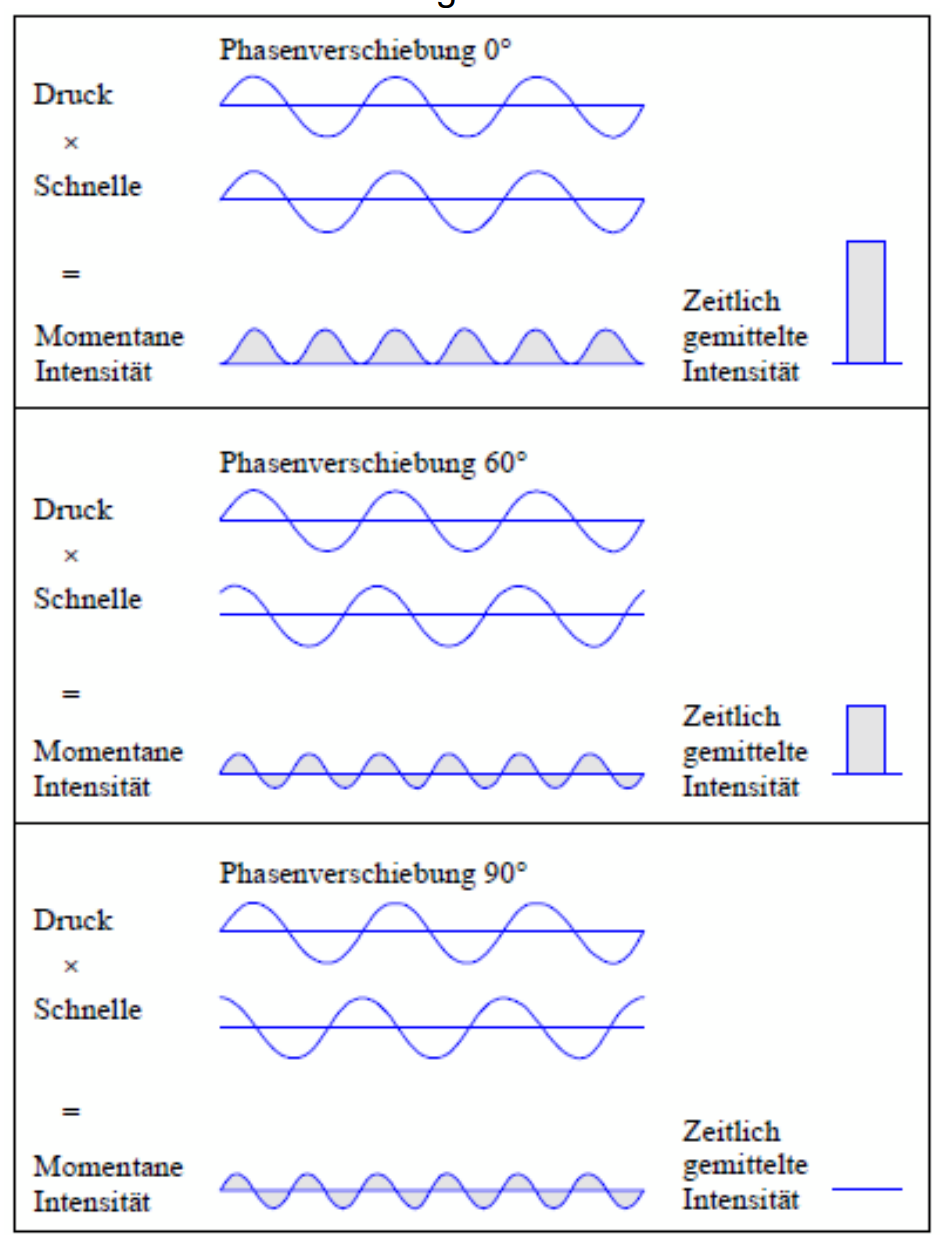
\includegraphics[scale=0.5]{papers/helmholtz/images/Schallintensitaet.png}
	\caption{Schallintensität Beispiel}
	\label{fig:Schallintensitaet}
\end{figure}

\begin{itemize}
	\item komplexe akustische Intensität: \\
	\begin{equation}
	\mathbf{I}_c ~(\mathbf{r}) = \underbrace{\mathbf{I}~(\mathbf{r})}_{\textit{aktive Intensität}} + \underbrace{j\,\mathbf{Q}~(\mathbf{r})}_{\textit{reaktive~Intensität}}
	\label{helmholtz:equationIntensitaetComplex}
	\end{equation}	
			
	\item Zeitlich gemittelte Intensität (aktive Intensität) \\
	\begin{equation}
	\mathbf{I}~(\mathbf{r}) = \frac{1}{T}\int_0^T \mathbf{I}_i(\mathbf{r},t)\,~\mathrm{d}t = \frac{1}{2}\Re\left\{P(\mathbf{r})~\mathbf{U}^*(\mathbf{r})\right\}
	\end{equation}
	
	\item aktive Intensität: \\
	\begin{equation}
	\mathbf{I} = \frac{P^2}{2P_0\omega}
	\label{helmholtz:equationAktiveIntensitaet}
	\end{equation}
	
	\item Reaktive Intensität: \\
	\begin{equation}
	\mathbf{Q}(\mathbf{r}) = \frac{1}{2}\Im\left\{P(\mathbf{r})~\mathbf{U}^*(\mathbf{r})\right\}
	\label{helmholtz:equationReaktiveIntensitaet}
	\end{equation}
	
\end{itemize}
